\section{Costs of Education} \label{appendix:education}

\noindent We account for short- and long-term components of education costs. The short-term components include savings due to reductions in special education and grade retention. The long-term components include the type and level of the highest educational attainment at age 30. We do not calculate costs of education beyond age 30 because we do not have data on the subjects' later educational attainment. Instead of forming a projection, we do not add further modeling uncertainty through this component and document that, at the national level, education beyond age 30 increases marginally. To document this, we use the  Panel Study of Income Dynamics (PSID) for a representative sample of individuals born between 1972 and 1982. \\

\noindent To estimate the costs of additional schooling, we combine various sources. Table \ref{tab:yearlyedu}  describes the yearly cost of education at every level and the age and duration for which these costs are incurred. We apply these costs additively up to the highest level of educational attainment by age 30. Pooling males and females, the treatment groups had on average higher attainment and incurred a greater cost of education. To find the present value of the difference between the treatment and control groups, we first order educational attainment per Table \ref{tab:yearlyedu}. We find a difference between the average educational attainment of the treatment groups (finish community college) and the average educational attainment of the control groups (start community college). This can be represented as a cost that is \$12,586 higher for the treatment groups than for the control groups, as in Table \ref{tab:yearlyedu}. The effect of the program on the educational attainment of females, however, is much greater than the effect on that of males.

\subsection{Measuring Lifetime Educational Attainment}

\noindent Follow-up data on educational attainment were collected for ABC and CARE subjects up to age 30, on average. This may not necessarily be an accurate measure of lifetime educational attainment. Thus, we perform an exercise using nationally representative data from the Panel Study of Income Dynamics (PSID) to assess educational attainment after age 30. Figure \ref{fig:psid-exercise} shows the results of our exercise. \\

\begin{center}
\begin{figure}[H] 
\caption{Additional Education After Age 30} \label{fig:psid-exercise}
\label{figure:youlabel}
\centering
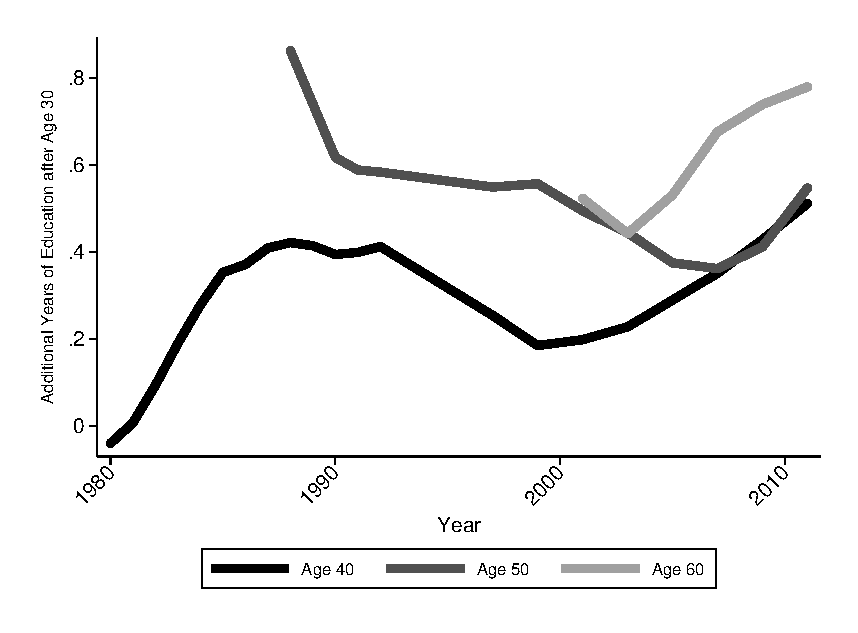
\includegraphics[width=.9\columnwidth]{AppOutput/Education/addeducfrom30.eps}
\floatfoot{
\footnotesize
Note: This plot uses data from the Panel Study of Income Dynamics (PSID) to display the mean years of education beyond the education level at age 30, by years. We report this value for ages 40, 50, and 60. The domain of the trends is a function of data availability, i.e. of longitudinal span in the data. Each yearly calculation uses cross-sectional weights to attain nationally representative statistics.
}
\end{figure}
\end{center}

\noindent Figure~\ref{fig:psid-exercise} displays the average additional years of education at ages 40, 50, and 60. The series have different spans due to restrictions in data availability. Individuals, on average, never go a year beyond their education at age 30. We assume that imprecision generated by not observing educational levels beyond age 30 is of second order, and do not project additional educational attainment.

\subsection{Cost of Education}
\noindent We apply the costs described in Table \ref{tab:yearlyedu} to subjects' educational attainment at age 30 to calculate the public and private costs of lifetime educational attainment. Costs up to high school are assumed to be public costs. \\

\begin{table}[H]
\caption{Yearly Individual Education Costs} \label{tab:yearlyedu}
\centering
\begin{adjustbox}{max width=\textwidth}
\begin{threeparttable}
\footnotesize
\begin{tabular}{C{3.5cm} C{1.5cm} C{1.5cm} C{2cm} C{6.5cm}}
\toprule
Schooling level & Ages & Duration (Years) & Yearly Cost &Attainment \& Notes\\ \midrule
K-11 & 6-16 & 10 &   \$9,113  & All subjects. Only 1 control individual dropped out before completing 9th grade; we assume completion up to 8th grade. \\
Grade 12 & 17-18 & 2 &  \$9,113  & Counted only for subjects who completed high school, 29:38 (control:treatment).\\ \\
GED (Started) & 19 & .5 &  \$155& GED is considered a one year program. No subjects identified as having starting a GED program without finishing.\\ \\
GED (Completed) & 19 & 1 & \$155 & 8:6 (control:treatment).\\ \\
Vocational or Technical Training (Started)& 19 & 1 & \$7,245 & 8:3  (control:treatment).\\ \\
Vocational or Technical Training (Completed)& 19-20 & 2 &  \$7,245 &  4:9 (control:treatment)\\ \\
Community College (Started) &   19 & 1 &  \$7,001 & 11:6 (control:treatment) \\ \\
Community College (Completed) & 19-20 & 2 &  \$7,001 & 9:8 (control:treatment)\\ \\
 College (Started)   &  19 & 1 &  \$7,685& Assume dropouts drop out at the end of the first year. 5:8 (control:treatment).\\ \\
 College (Completed) &  19-22 & 4 & \$11,886 & 3:8 (control:treatment)\\ \\
Graduate School (Started) & 23 & 1 &  \$9,704& Assume dropouts drop out at the end of the first year. 2 treated individuals.\\ \\
 Finished Masters &  23-25 & 2 &  \$9,704& 1 treated individual\\ \\
 Finished PhD & 23-26 & 4 & \$9,704 & 1 treated individual\\ \\
 \midrule
 Grade Retention& NA & 1 &\$9,113 & \\ \\
 Special Ed.& NA & 1 &  \$11,705  & \\ 
 \bottomrule
 \end{tabular}

\centering
\begin{tablenotes}%[para,flushleft]
\scriptsize
\item Sources: \citet{Snyder_Willow_2012_BOOK_NCES}; \citet{Hoenack_Weiler_1975_JHR}; \cite{Dhanidina_Griffith_1975_AEQ}; \cite{Freeman_1974_Occupational-Training_RES}. \\
 Note: This table reports the yearly cost and duration of each type of education, as well as the ages for which we evaluate them.  All amounts are inflated to 2014 USD.
We show the number of subjects who identified themselves as being in each education category (total number of respondents: 101/114). To compute the total cost of education for a subject, we applied these costs additively up to the highest level of educational attainment. Only K-12 education, special  education, and grade retention costs account for deadweight loss. Because it gives costs that are applied across many years, this table does not show their present discounted value.
\end{tablenotes}
\end{threeparttable}
\end{adjustbox}
\end{table}

\subsection{Non-monetary Benefits of Education}

\noindent There are many social and non-monetary benefits of education that our analysis cannot capture. These benefits impact the individual's quality of life, the general well-being of society through positive peer effects as well as fewer costs and negative externalities, and even the well-being of future generations. Documenting them all may be impossible, but we briefly review some major benefits in this section. \cite{Vila_2000_Non-Monetary-Benefits-Education} documents private benefits with external effects, such as health (increases in longevity and better nutrition and preventative care choices). Higher education is also associated with decreased fertility rates linked with improved infant health and lower mortality rates. Moreover, higher education not only improves labor outcomes with respect to employment prospects and salary, but also with regard to how individuals perceive work and leisure, with more education leading to increased satisfaction from leisure. Furthermore, higher education is linked with better savings behavior and higher rates of return on savings. Higher education is also connected with social stability---better education promotes good citizenship and creates communities that are less likely to experience violent social conflict.\footnote{\citet{Lochner_2011_Handbook} or \citet{Lochner_2011_NBER}.}